% -------------------------------------------------------------------------------------------------
% Definitionen
% -------------------------------------------------------------------------------------------------
\documentclass[
    fontsize=12pt,                      % Schriftgröße 12 pt
    paper=a4,                           % Seitengröße A4
    twoside=off,                       % zweiseitiger Druck
    DIV=15,                             % Seiteneinteilung
    BCOR=12mm,                          % Bindekorrektur
    headings=normal,                    % normal große Überschriften
    headsepline=false,                   % Trennlinie unter der Kopfzeile
    footsepline=false,                  % Trennlinie über der Fußzeile
    headinclude=true,                   % Kopfzeile zählt zum Textkörper
    footinclude=false,                  % Fußzeile zählt nicht zum Textkörper
    toc=listof,                         % Verzeichnisse der Gleitumgebungen ins Inhaltsverzeichnis
    toc=bib,                            % Literaturverzeichnis ins Inhaltsverzeichnis
    chapterprefix=false,                % vor Kapitelnummern steht "Kapitel"
    appendixprefix=false,               % vor Anhangüberschriften steht "Anhang"
    numbers=noendperiod,                % Keinen Punkt hinter die letzte Zahl eines Kapitels (auch bei Anhang)
    captions=tableabove,                % Tabellenüberschriften setzen
    footnotes=multiple,                 % Erkennung von mehreren Fußnoten hintereinander
    bibliography=oldstyle,              % Literaturverzeichnis: openstyle oder oldstyle
    draft=false,                        % Entwurfsstadium
]{scrreprt}


% Paket Includes
% ----------------------------
\usepackage[T1]{fontenc}                % deutsche Umlaute und Sonderzeichen
\usepackage[utf8]{inputenc}             % Umlaute koennen direkt im Quelltext stehen
\usepackage[ngerman]{babel}             % neue deutsche Rechtschreibung 
\usepackage{lmodern}
\usepackage{graphicx}                   % Bilder einfügen
\usepackage{tabularx}                   % Tabellen mit fester Breite und variabler Spaltenbreite
\usepackage{array,longtable}            % Tabellen mit Seitenumbruch
\usepackage{booktabs}                   % bessere horizontale Linien in Tabellen
\usepackage{array,ragged2e}             % mehr Spaltentypen in Tabellen und neue Spaltentypen
\usepackage{dcolumn}                    % Spalten am Dezimaltrenner ausrichten
\usepackage{amsmath}
\usepackage[                            % Unterabbildungen mit folgenden Parametern:
            font=footnotesize,          % kleine Schrift
            labelfont={sf,bf},          % Labels fett und serifenlos
            textfont={sf},              % Text serifenlos
            format=hang,                % hängender Einzug
           ]{caption}
\usepackage{float}      
\usepackage{hyperref}                   % URL links     
\usepackage{xcolor}  


\definecolor{mygreen}{rgb}{0,0.6,0}
\definecolor{myred}{rgb}{0.7529,0.3137,0.3019}


\newcommand{\Farbcode}[1]{\texttt{\textbf{\textcolor{myred}{#1}}}}


% Kopf- und Fußzeile
% ----------------------------
\usepackage{scrlayer-scrpage} 
\setkomafont{pagehead}{\sffamily\small}
\setkomafont{pagefoot}{\sffamily\small}
%\automark{chapter}
\lohead{Modul Embedded Systems 2 -- Steuergeräte, Vernetzung, Software} \cohead{} \rohead{Übung 2-2}
\lofoot{\includegraphics[height=10pt]{Figures/HSMW-Logo-klein} HS Mittweida, INW, Prof. Thomanek}
\cofoot{} \rofoot{\thepage}

\pagestyle{headings}
\renewcommand*{\chapterpagestyle}{headings}% Nicht zu empfehlen, aber du willst das offenbar trotzdem.


\setcounter{secnumdepth} {3}
\addto\captionsngerman{\renewcommand{\figurename}{Abb.}}    % Verwende Abb. x.x anstatt Abbildung x.x
\renewcommand{\thefigure}{\arabic{figure}}
% -------------------------------------------------------------------------------------------------
% Dokument
% -------------------------------------------------------------------------------------------------

\begin{document}


\chapter*{Übung 2-2 -- Echtzeitbetriebssysteme}

\section*{Nichtpreemptiver Scheduler}
\textbf{(a.)}
\vskip 0.2cm
\noindent
Schreiben Sie für den Arduino einen einfachen \textbf{nichtpreemptiven Scheduler} (\Farbcode{sched.h}, \Farbcode{sched.cpp} -- siehe Template-Dateien in OPAL) mit den folgenden Anforderungen:
\begin{itemize}
\item Der Scheduler besitzt einen Puffer mit einer maximalen Anzahl handelbarer Tasks (z.B. 10) 
\item Jede Task besitzt einen \textbf{\emph{Task Control Block}}, bestehend aus (vgl. Bild)
\begin{itemize}
\item Zeiger zur Taskfunktion
\item (Optional: Zeiger auf mögliche Argumente der Taskfunktion)
\item Zykluszeit
\item Aktivierungszeitpunkt
\item Tasktyp (\Farbcode{NOP, IDLE, ONCE, CYCLIC})
\end{itemize}

\begin{figure}[H]
	\centering
	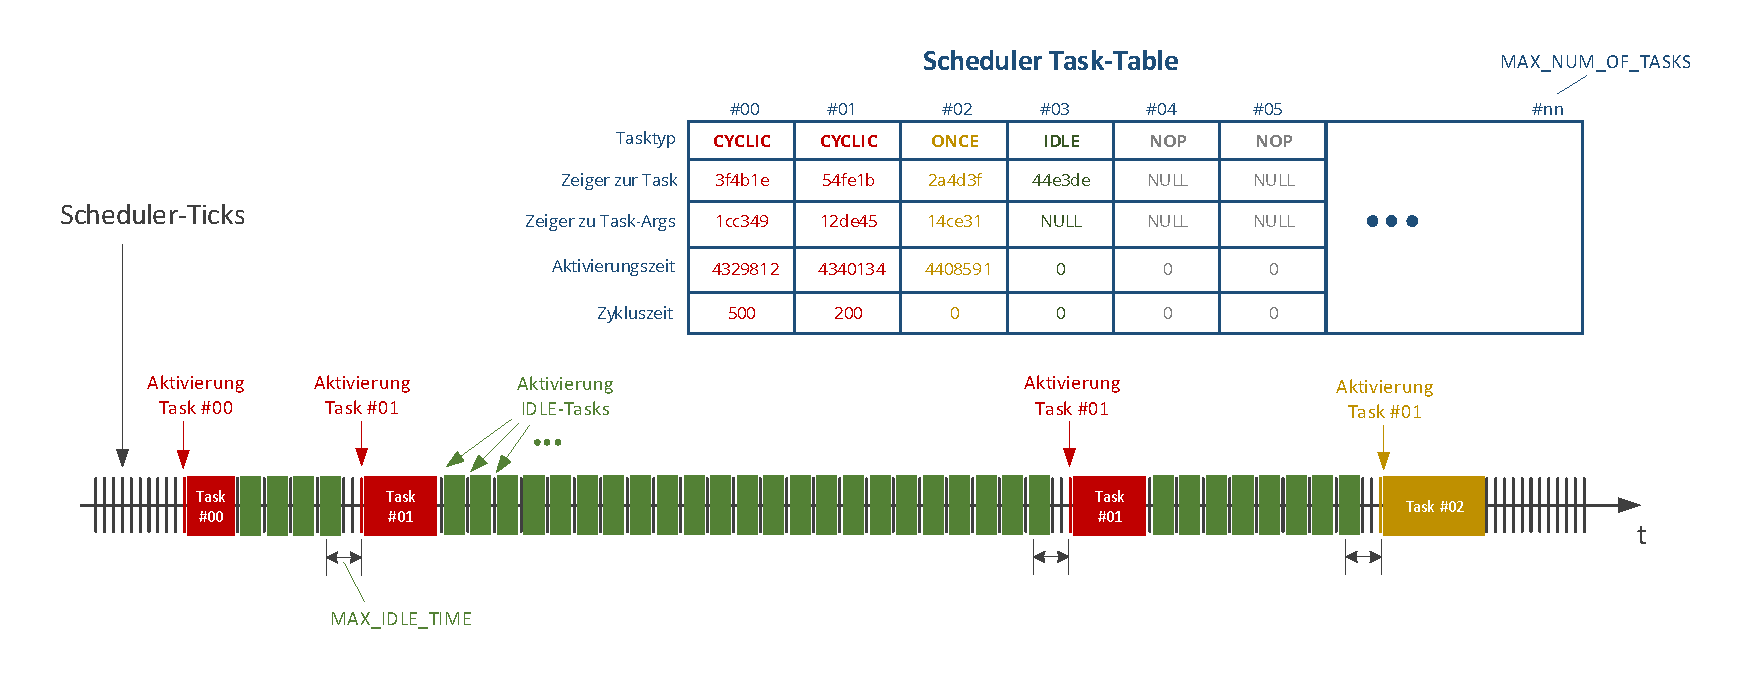
\includegraphics[width=\textwidth]{Figures/Scheduler}
\end{figure}

\item Der Scheduler ruft in Abhängigkeit des Typs und der Zyklus- und Aktivierungszeit die aktiven Tasks im Puffer entsprechend auf  
\item Verwenden Sie als Zeitbasis die Funktion \Farbcode{millis()} der Arduino-Bibliothek -- Sie liefert einfach einen aktuellen Zähler zurück (Zeit in ms seit Reset), der durch einen Interrupt aller 1024 $\mu$s inkrementiert wird
\item Liegt keine Aktivierung einer regulären Task unmittelbar bevor, werden die möglichen IDLE-Tasks aufgerufen

\item \textbf{Öffentliche Schnittstellen} (Funktionen) zur Anwendung:
\begin{itemize}
\item Initialisieren des Schedulers 
\item Ausführen des Schedulers
\item Hinzufügen einer Task
\item Löschen einer Task
\end{itemize}

\end{itemize}

\vskip 0.5cm
\noindent\textbf{(b.)}
\vskip 0.2cm
\noindent
Schreiben Sie ein einfaches Anwendungsprogramm für den Arduino (siehe Template-Sketch in OPAL), das drei periodische Tasks unterschiedlicher Zykluszeiten definiert
\begin{itemize}
\item \Farbcode{Task100ms}
\item \Farbcode{Task500ms}
\item \Farbcode{Task1000ms}
\end{itemize}
\noindent
Um die Aufruffrequenzen der Task zu prüfen, soll mit deren Durchlaufen \textbf{je eine eigene LED ein- bzw. ausgeschaltet} werden, wie in der folgenden Abbildung aufgebaut.

\begin{figure}[H]
	\centering
	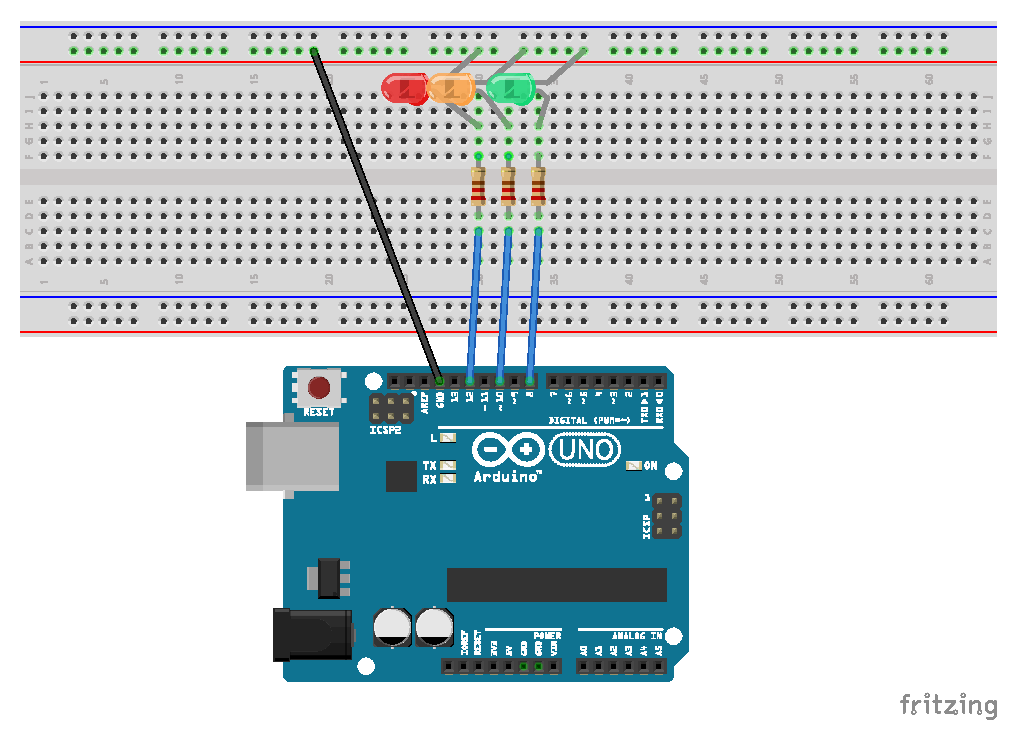
\includegraphics[width=0.8\textwidth]{Figures/Scheduler_Steckplatine}
\end{figure}


\end{document}